Um das in Abschnitt \ref{subsec:dither sampling} vorgestellte \textit{Dither Sampling} zu realisieren
benutzen wir für den temporalen Algorithmus \ref{ch:Temporaler Algorithmus} diese im Folgenden vorgestellten
\glqq nachträglichen\grqq Annahmen \cite{hal02158423}. 
A Posteriori sind Sie in dem Sinne, als das wir die Annahmen szenenabhängig machen und Sie anhand 
von bereits erstellten Pixelwerten formulieren. 

\subsection{Theoretische Grundlage}

Im Kapitel \nameref{ch:Content1:sec:Path Tracer} haben wir gesehen, dass 
wir den Wert eines Pixels (i,j) klassischerweise mit einem zufälligen
Startwert durch eine Monte-Carlo Integration erhalten. Wir betrachten im
Folgenden eine (theoretische) Menge von allen möglichen Werten eines 
Pixels, welche durch alle möglichen Startwerte generiert wurde.
In Abbildung \ref{eq:Pixel Schätzung Wahrscheinlichkeitsdichtefunktion} ist die Wahrscheinlichkeitsdichtefunktion
$h_{ij}$ aufgetragen, als eine Funktion über alle möglichen Werte 
$I_{ij}$ eines Pixels (i,j).

\begin{equation}\label{eq:Pixel Schätzung Wahrscheinlichkeitsdichtefunktion}
    H_{ij}([I_{Anfang},I_{Ende}]) = \int_{I_{Anfang}}^{I_{Ende}} h_{ij} dI
\end{equation}

Verfolgt man beispielhaft die Werte eines Pixels über neun Bilder bei unseren \nameref{ch:Content1:sec:Path Tracer}, 
so ergibt es sich zur Anschauung wie folgt:

\begin{figure}[H]

    \begin{subfigure}{\textwidth}
        \centering 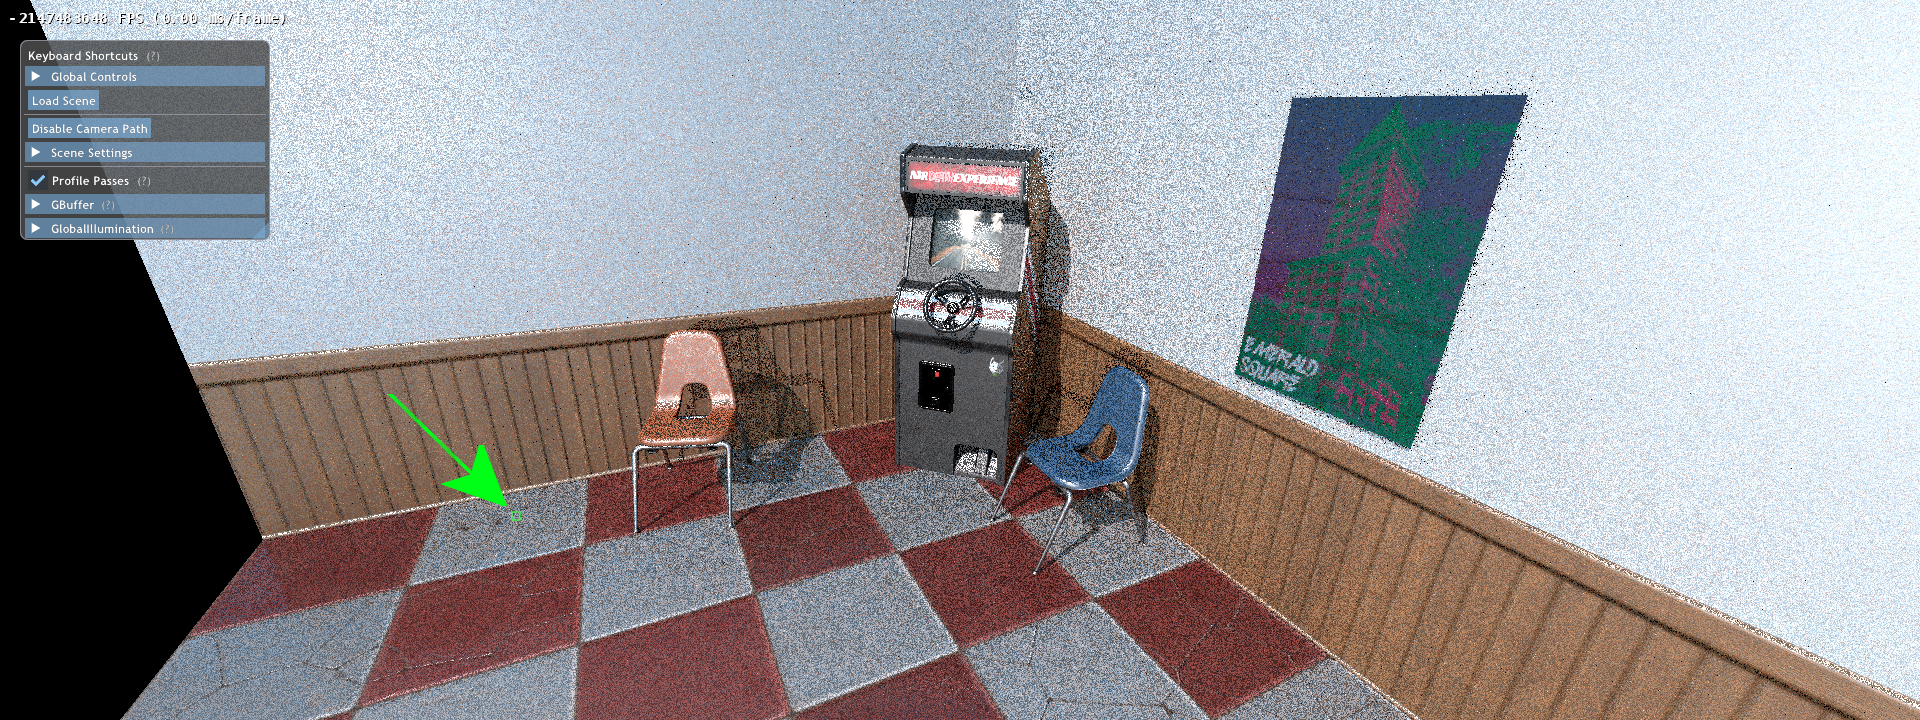
\includegraphics[width=0.6\linewidth]{content/TemporalerAlg/Bilder/APosteriori/frame_t_whitenosie2.0.png} 
        \caption{Szenenausschnitt}
        \label{fig:szene_pixel_position_512x512}
    \end{subfigure}

    \begin{subfigure}{0.5\textwidth}
        \centering 
\includegraphics[width=0.6\linewidth]{content/TemporalerAlg/Bilder/APosteriori/pixel_512x512_strip.png} 
        \caption{Werte des Pixels an Position 512x512 im zeitlichen Verlauf (grüner Pfeil)}
        \label{fig:ausschnitt_pixelstrip}
    \end{subfigure}
    \begin{subfigure}{0.5\textwidth}
            \centering
            \def\svgwidth{\columnwidth}
            \import{content/TemporalerAlg/Bilder/APosteriori/}{histogram_of_estimates.pdf_tex}
            \caption{Histogram der Pixelschätzungen}
            \label{pic:histogramOfEstimates}
    \end{subfigure}
        \caption{Pixelwerte an Position 512x512(grüne Markierung) in aufeinanderfolgenden Zeitschritten}
        \label{fig:Pixelwerte}

\end{figure}

Betrachten wir die theoretische, praktisch nicht umsetzbare Menge aller möglichen Werte. 
Mit dieser Menge haben wir ein vollständiges Histogramm. Dies bedeutet wiederrum, dass das Erzeugen eines 
Pixelwertes nichts anderes bedeutet, als eine zufällige Wahl anhand der impliziten
Wahrscheinlichkeitsdichtefunktion. Wir können als einem zufälligen Anfangswert einen konkreten 
Pixelwert zuteilen und eine umkehrbare Funktion definieren \ref{eq:inverse Funktion}. 

Daraus lässt sich die Gleichbedeutung zweier Aussagen begründen:
Das Rendern des Pixels (i,j) und das Wählen eines Pixelswertes $I_{ij}$
von unser zuvor formulierten Wahrscheinlichkeitsdichtefunktion $h_{ij}$.

\begin{equation}\label{eq:inverse Funktion}
    I_{ij} = H_{ij}^{-1}(x), x \in [0,1]
\end{equation}

\par

\textbf{Fazit}: Falls $x \in d_{ij}$, wobei d eine korrelierte Zahlenfolge, die einer 
\nameref{ch:Content1:sec:blue noise} Verteilung entspricht, folgt aus der bijektiven
Natur der Gleichung \ref{eq:inverse Funktion} eine \nameref{ch:Content1:sec:blue noise} 
Fehlerverteilungen im Bildraum. 

Anmerkung: Das Dies nur theoretisch möglich und gerade für Echtzeitanwendungen nicht umsetzbar ist, 
folgt eine praktikable Formulierung!

\subsection{Praktische Durchführung}

Die Berechnung des vollständigen Histogramms ist für eine Echtzeitanwendung
zu kostenintensiv. Stattdessen könnte man auch die dadurch beanspruchte 
Rechenleistung auf z.B mehrere Samples pro Pixel verteilen und dadurch eine 
Steigerung der Bildqualität erreichen!
Stattdessen werden wir in dem temporalen Algorithmus (siehe \cite{hal02158423})
das Histogramm mit dem vorherigen Bild approximieren. 
Die Approximation des Histogramms erfolgt dadurch mit dem $Frame_{t}$ 
für $Frame_{t+1}$. Daher ist eine getroffene Annahme, um die gute Funktionalität des 
Algorithmus zu garantieren, eine nicht zu schnelle Bewegung der Kamera.
Außerdem werden für das Histogramm eines Pixels seine umliegenden benachbarten Pixel gewählt.
Daher ist eine weitere getroffene Annahme, um die gute Funktionalität des 
Algorithmus zu garantieren, eine möglichst homogene Fläche. 
Offensichtliche Konsequenzen dieser blockweisen Verarbeitung sind schlechte blue noise 
Fehlerverteilungen im Bildraum bei sich stark ändernden Bildausschnitten
(so z.B. bei Objektkanten), da dort die Annahme, dass eine ähnliche Oberfläche
zur Farbgebung beiträgt verletzt wird.

\begin{figure}[H]
    \centering
    \begin{subfigure}[b]{0.4\textwidth}
        \centering 
\includegraphics[interpolate=false, width=\linewidth]{content/TemporalerAlg/Bilder/APosteriori/homogener_ausschnitt_blocksize.png}
        \caption{homogener Pixelblock}
        \label{fig:homogener Pixelblock}
    \end{subfigure}
    \begin{subfigure}[b]{0.4\textwidth}
        \centering 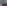
\includegraphics[interpolate=false,width=\linewidth]{content/TemporalerAlg/Bilder/APosteriori/inhomogener_ausschnitt_blocksize.png}
        \caption{inhomogener Pixelblock}
        \label{fig:Inhomogener Pixelblock}
    \end{subfigure}

    \caption{Pixelblöcke bei (in-)homogenen Flächen}\label{fig:Pixelblöcke}
\end{figure}

In Abbildung \ref{fig:Inhomogener Pixelblock} sind die benachbarten Pixel eine gute 
Approximation des jeweiligen Pixels, wohingegen in Abbildung \ref{fig:homogener Pixelblock}
die benachbarten Pixel dies nicht sind.